\documentclass[titlepage]{article}
\usepackage{graphicx} % Required for inserting images

\usepackage[T1]{fontenc}
\usepackage{tgbonum}

\def\companyName{shmap}

\begin{document}

\begin{titlepage}
    \begin{center}
        \vspace*{1.5cm}

        {\fontfamily{phv}\selectfont
            {\Huge \companyName}
        }

        \vspace{0.5cm}
            {\large Convenient, united frontend for connecting\\
        stores, brands and customers}
            
        \vspace{1.25cm}

        \textbf{Project Group E1} \\
        {\normalsize Viktor Jernberg (vi6832je-s@student.lu.se)\\Thomas Dellwik (th5144de-s@student.lu.se)\\Nils Reberg (ni7877re-s@student.lu.se)\\Nicolas Jaua Otero (ni1407ja-s@student.lu.se)\\Marina Fridh-Cardoso (ma0448fr-s@student.lu.se)\\Erik Nicander (er0811ni-s@student.lu.se)}

        \vspace{1.25cm}

        
\includegraphics[width=0.45\textwidth]{logo_gradient.png}
       
        \vspace{1.5cm}

        {\Large Lund, Sweden}

        \vspace{0.5cm}
        
        {\Large 2024}\\
            
    \end{center}
\end{titlepage}

\section{Executive Summary}
Our product provides a new and effective way for in-store shoppers to navigate smoothly through any storefront. A mobile application with a streamlined and effective indoor navigation system that guides users through stores, allowing large shopping lists to be completed in quicker, more comfortable ways for the user. 

For customers, i.e large retail stores, we provide valuable data on user activity within the stores, allowing them to evaluate under/over-utilized areas of their locations while enabling effective advertisement of select products based on shopper data and interests. 

Our team, containing experienced algorithm developers and with previous experience in the retail industry, are suited to create a product that understands both what stores and store-goers are wanting for in the current system.

\section{Management team}
Our team consists of six computer science students who attend Lund University. We are currently in our third year of our studies and have learned a great deal about software and programming. Even though we study together, the members of the team have varying experiences that are relevant for this project.

The members are: Thomas Dellwik, Marina Fridh-Cardoso, Nicolas Jaua Otero, Viktor Jernberg, Erik Nicander and Nils Reberg. The different relevant experiences that the members have will help with early development and serves as a great base for us to get started. For example: Nicolas has previously worked with startups and has designed apps, Erik is great at design concepts and has done graphic design, and Viktor has worked a management role at a grocery store which is relevant because grocery stores are the target customer.

The main concern about competence missing from the team  is legal education and possibly leadership experience. If we could have a person with legal knowledge in our team, our team would essentially be complete as a startup.

\section{Business Model}
The main customer segment of our product are retail and grocery stores, and the contingent of shoppers who appreciate assistance, 
guidance or finding deals using cloud services. 
Many customers of stores have difficulties in finding where items in aisles are.
Unlike current solutions, which give minimal or no information to the consumer on where to go for various items,
our solution aims to instead give the consumer the ability to find items with a mobile solution,
letting them obtain information of product positions without having to actively seek them out.
In addition, the staff requirement of providing information to store customers would be greatly relaxed.

Usage and improvement of our product are tightly interconnected, as by user data such as store customer positions over time 
and user-provided map complementary data, our product improves. 
Unlike other solutions, our model can also combine the data from different model consumers, 
facilitating a high potential for growth.

By initially releasing our product for a lower price than a projected market price for a similar solution,
a market position as a leader in the product space would be obtained.
After obtaining a larger market share, a revenue stream by advertisements, 
licensing fees and selling the user data would be lucrative.

\begin{figure}[h]
    \centering
    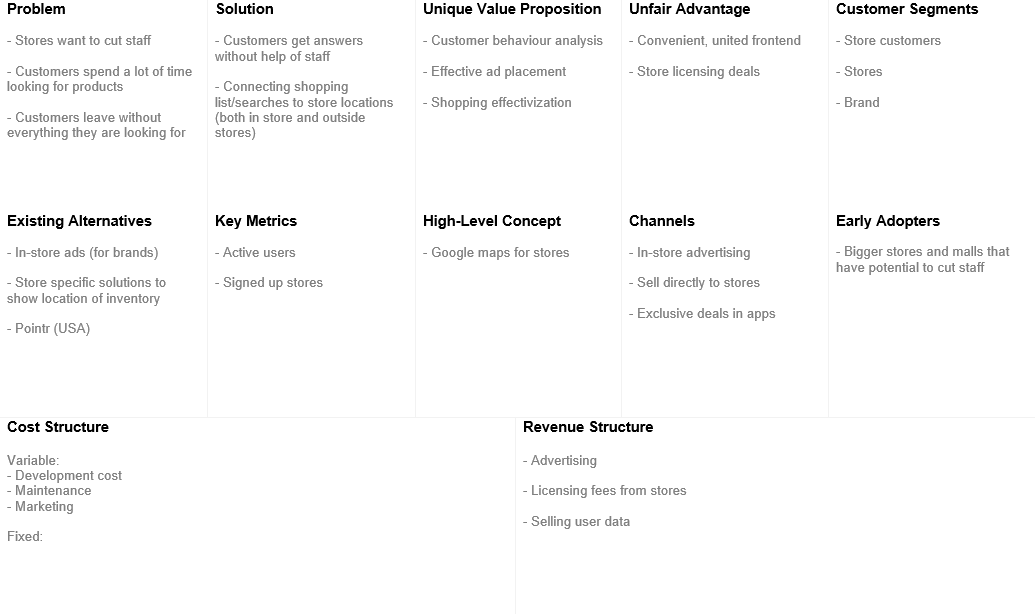
\includegraphics[width=1\textwidth]{lean model canvas.png}
    \caption{Lean model canvas describing \companyName's business model}
    \label{fig:enter-label}
\end{figure}

\section{Market Analysis}
Our product would be aimed at in-store shoppers, people who want help getting around different stores and getting the best possible deals for what they are searching for. There are multiple current alternatives that cover part of what we aim for. For example, many supermarket stores have their own apps that show weekly deals, searching for products, among other things. Other apps like Tiendeo offer the possibility of seeing the catalog of discounts in nearby stores in your area. And the stores themselves usually display their own discounts and offer physical catalogs with their offers. 

Though this helps when searching for deals, it doesn’t help customers find their way within the store, where they would rely on looking around, checking the signs or asking for help from the store personnel. Pointr offers the possibility of indoor positioning, but it hasn’t reached the Swedish market, and it’s limited to countries like the US and the UK. 

Our product has the ability of combining the side of navigation within the store, optimizing routes according to items or shopping lists, plus promoting the user with deals and offering the option to compare product prices in different stores from the comfort of a single app.

For our initial market we would aim to partner with some individual stores in limited locations to show both users and customers, like supermarket chains, the possibilities our app offers. We would start with a smaller city, like Lund, and promote the app in front of the stores we’d be partnered with. We would aim our product mainly to bigger families, who want to optimize the time they spend in stores and the amount of money they spend on products.

\section{Implementation plan}

\section{Risk assessment}

\section{Contribution statement}
Thomas Dellwik: Part of group brainstorming and discussions when forming our business idea and MOM-test questions. Responsible for writing the Business model section in the first draft of the report. Spent around 5 hours total. \\
\\
Marina Fridh-Cardoso: Participated in discussions in regards to formulating and refining our business idea. Strengths and weaknesses, how to create value for both customers (retailers) and users. Active in planning and executing MOM-test. Together with team members filled out the Lean Canvas. Formalia and structure of report draft. Approx.  5 hours of work. \\
\\
Nicolas Jaua Otero: Active part in discussions and planning of business idea and strategy. Contributed to MOM-test planning and execution. Wrote the Market analysis section of the report. About 5 hrs work.\\
\\
Viktor Jernberg: Took part in brainstorming, refining and planning business idea and business strategy, following the Lean Canvas Model. Active part of planning and executing the MOM test. Responsible for writing first draft of Management team section. About 5 hours.\\
\\
Erik Nicander: Participated in group discussions and planning, attended seminars and group planning meetings. Took an active role in developing our business idea and in fleshing out the business strategy and filled in the Lean Canvas. Approximately 5 hours of work in total.\\
\\
Nils Reberg: Took on a leading role in coming up with and refining the business idea and strategy, and completing Lean Canvas.  Involved in planning and execution of MOM-test. Author of the Executive summary section. Total time about 5 hrs spent.\\


\end{document}
